\section{Minutiae Identification with Verifinger Software}

\subsection{ROC Curve from Zhonghao's ISO Files}

\begin{figure}[h]
    \centering
    \subfloat[]{
    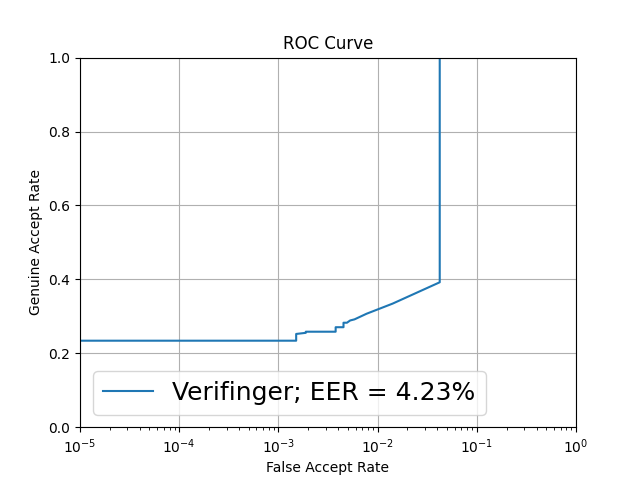
\includegraphics[width=2.5in]{Figure/26-08-2022/zhonghao-all-to-all.png}
    \label{zhonghao-all-to-all}}
    \subfloat[]{
    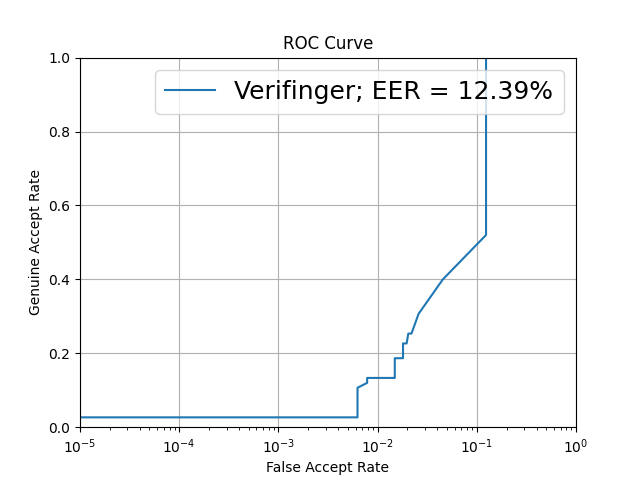
\includegraphics[width=2.5in]{Figure/26-08-2022/zhonghao-leave-one-out.png}
    \label{zhonghao-leave-one-out}}
    \caption{ROC curve from Zhonghao's iso files. (a) using the all-to-all protocol? (b) using leave-one-out protocol.}
    \label{zhonghao}
\end{figure}

Firstly, I used the generated "iso" files from Zhonghao to draw ROC curve (Fig. \ref{zhonghao}). But I found two problems, one is that he used \textcolor{red}{all-to-all protocol? which have numsubjects x samplesofeachsubject x samplesofeachsubject genuine matching scores, and numsubjects x (numsamples -1) x samplesofeachsubject x samplesofeachsubject imposter matching scores.} Therefore the ROC curve can be shown as the Fig. \ref{zhonghao-all-to-all} with 4.23\% EER value. And I changed the protocol to leave-one-out protocol, each sample gets the minimal matching score (genuine scores: numsubjects x samplesofeachsubject, imposter scores: numsubjects x (numsamples -1) x samplesofeachsubject). The ROC curve as shown on the Fig. \ref{zhonghao-leave-one-out} with 12.39\% EER value. \textcolor{red}{The rest experiment will follow the leave-one-out protocol to get the genuine and imposter matching scores.} The another problem is the name of minutiae text files. \textcolor{red}{His file name was misnamed and different samples of the same person did not match up, so it resulted in a low match score between different samples of the same subject}.

\subsection{Processing Finger Nail Blood Vessel Minutiae Result Text File}
Firstly, I sorted all the endings and bifurcations according to their respective confidence levels, and subsequently deleted them from the lower confidence levels if they needed to be deleted. The second step is to rename all the files, with the nth sample of subject $x$ renamed as $x_n.txt$. \textcolor{red}{ Because the renaming method of Zhonghao is wrong, it result in, for example, zero matching score for different samples of the same subject.} In the third step, if the (x,y) and angle need to be changed in range, normalisation is performed. Finally, transform there text file to the iso files as the input of VefiyCPP.exe.

\textcolor{red}{Notes: The total number of ending points and bifurcations should not exceed 255; When the angle range changes, it should be (0, 360]; The number of bifurcations must not exceed 62. Otherwise, the VerifyCPP.exe will report an error with (ERROR: NError: (-15) Unexpected end of stream.)}

\subsubsection{Using Original Minutiae Results}
I used the original minutiae (x,y,angle,class,qulity) value to generate iso files and then used the VerifyCPP.exe to generate matching scores. As for the protocol, I use the leave-one-out protocol (same as my finger knuckle experiment protocol). At this step, I just changed the number of ending points and bifurcations as the Table \ref{original-text-table}, and the corresponding ROC curve as shown on the Fig. \ref{original-text}.

\begin{table}[h!]
    \centering
    \caption{}
    \begin{tabular}{cccccc}
    \hline
    Angle Range & (x,y) Range  & Minutiae                     & EER     & DI   & Figure \\ \hline
    {[}0, 180)  & (1920, 1080) & Only 255 Ending              & 0.00\%  & 3.47 & Fig. \ref{only-ending-255}  \\
    {[}0, 180)  & (1920, 1080) & Only 128 Ending              & 0.94\%  & 3.6  & Fig. \ref{only-ending-128}  \\
    {[}0, 180)  & (1920, 1080) & Only 64 Ending               & 0.86\%  & 3.35 & Fig. \ref{only-ending-64}  \\
    {[}0, 180)  & (1920, 1080) & Only 32 Ending               & 4.24\%  & 2.12 & Fig. \ref{only-ending-32}  \\
    {[}0, 180)  & (1920, 1080) & Only 16 Ending               & 16.20\% & 1.5  & Fig. \ref{only-ending-16}  \\
    {[}0, 180)  & (1920, 1080) & Only 62 Bifurcation          & 14.67\% & 1.45 & Fig. \ref{only-bifurcation-50}  \\
    {[}0, 180)  & (1920, 1080) & Only 32 Bifurcation          & 22.67\% & 1.07 & Fig. \ref{only-bifurcation-32}  \\
    {[}0, 180)  & (1920, 1080) & Only 16 Bifurcation          & 26.35\% & 0.79 & Fig. \ref{only-bifurcation-16}  \\
    {[}0, 180)  & (1920, 1080) & Ending: 193; Bifurcation: 62 & 0.47\%  & 3.73 & Fig. \ref{ending-193-bifurcation-62}  \\
    {[}0, 180)  & (1920, 1080) & Ending: 96; Bifurcation: 32  & 1.02\%  & 3.65 & Fig. \ref{ending-96-bifurcation-31} \\
    {[}0, 180)  & (1920, 1080) & Ending: 48; Bifurcation: 15  & 1.33\%  & 2.87 & Fig. \ref{ending-48-bifurcation-15} \\
    {[}0, 180)  & (1920, 1080) & Ending: 24; Bifurcation: 7   & 11.14\% & 1.65 & Fig. \ref{ending-24-bifurcation-7} \\ \hline
    \end{tabular}
    \label{original-text-table}
\end{table}

\begin{figure}[h!]
    \centering
    \subfloat[]{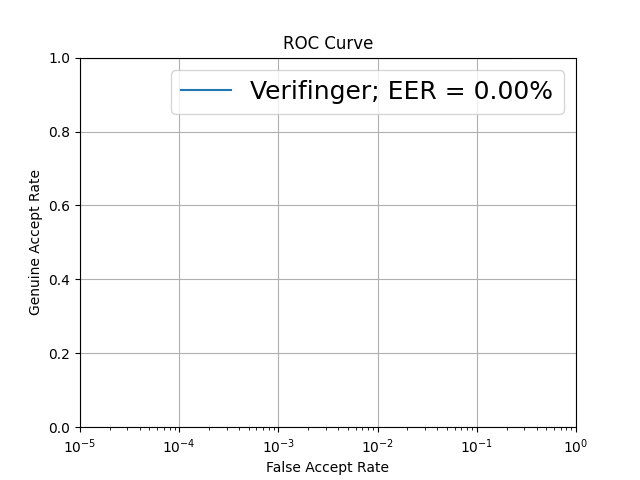
\includegraphics[width=1.74in]{Figure/26-08-2022/online-ending-255.png}%
    \label{only-ending-255}}
    \subfloat[]{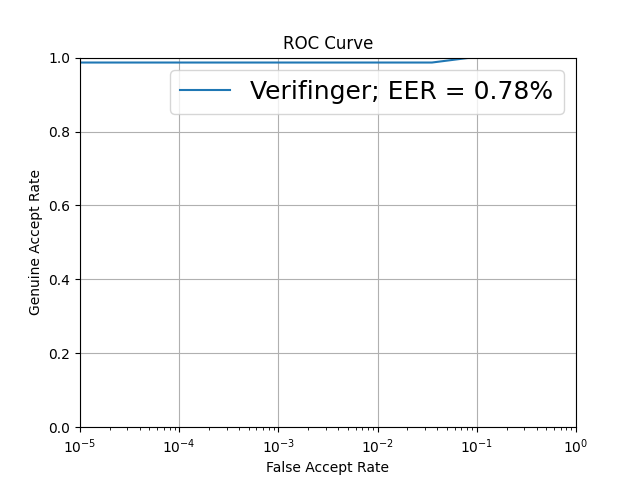
\includegraphics[width=1.74in]{Figure/26-08-2022/online-ending-128.png}%
    \label{only-ending-128}}
    \subfloat[]{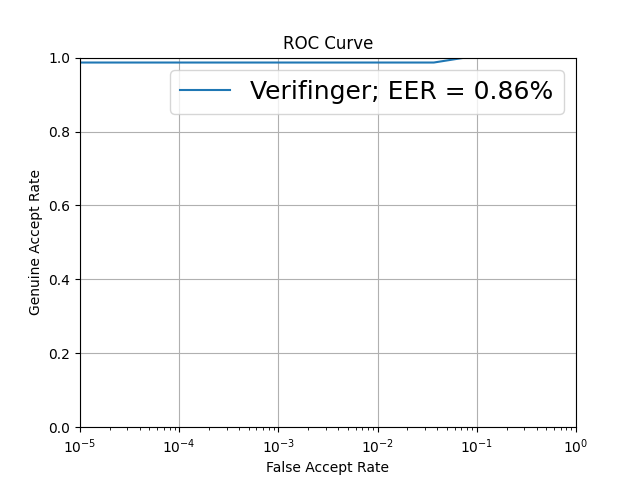
\includegraphics[width=1.74in]{Figure/26-08-2022/online-ending-64.png}%
    \label{only-ending-64}}
    \subfloat[]{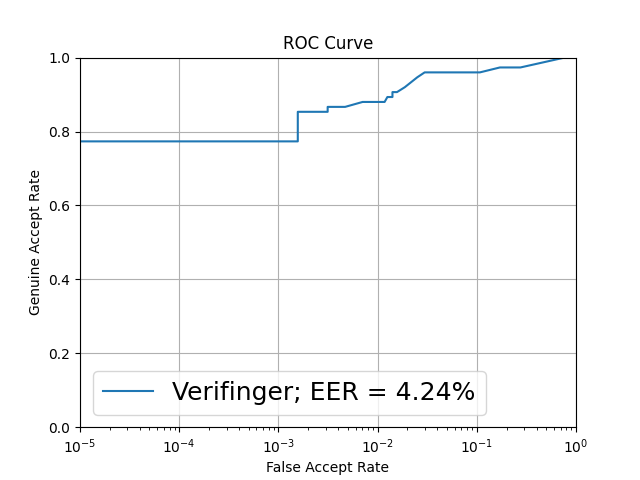
\includegraphics[width=1.74in]{Figure/26-08-2022/online-ending-32.png}%
    \label{only-ending-32}}

    \subfloat[]{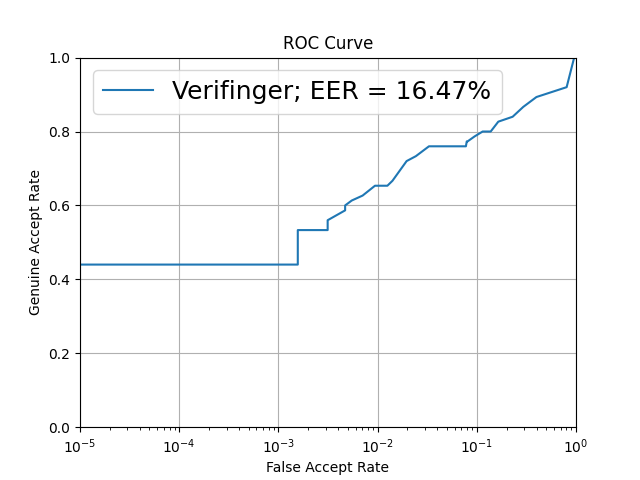
\includegraphics[width=1.74in]{Figure/26-08-2022/online-ending-16.png}%
    \label{only-ending-16}}
    \subfloat[]{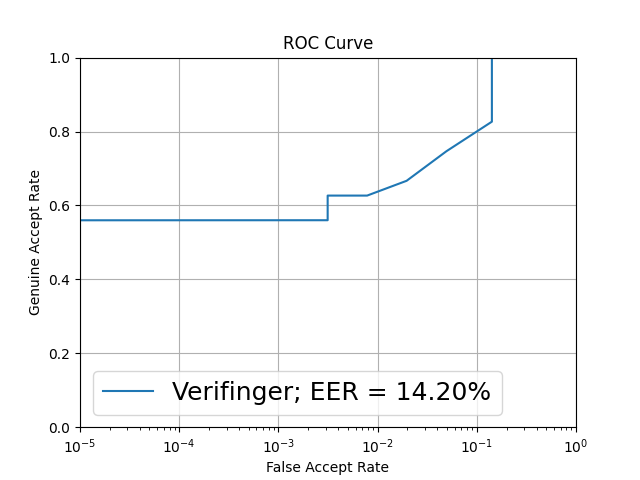
\includegraphics[width=1.74in]{Figure/26-08-2022/online-bifurcation-50.png}%
    \label{only-bifurcation-50}}
    \subfloat[]{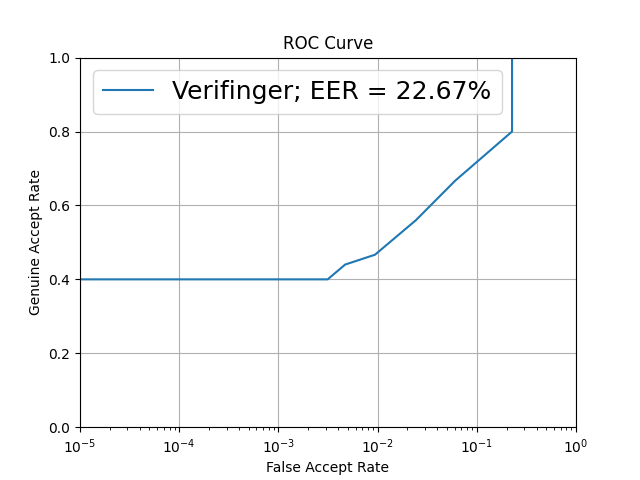
\includegraphics[width=1.74in]{Figure/26-08-2022/online-bifurcation-32.png}%
    \label{only-bifurcation-32}}
    \subfloat[]{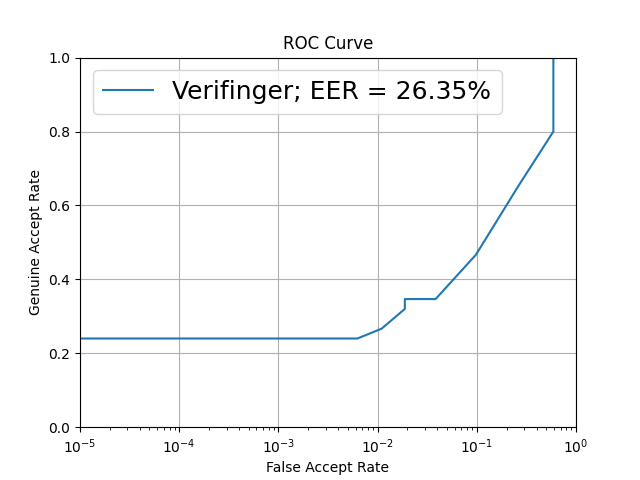
\includegraphics[width=1.74in]{Figure/26-08-2022/online-bifurcation-16.png}%
    \label{only-bifurcation-16}}

    \subfloat[]{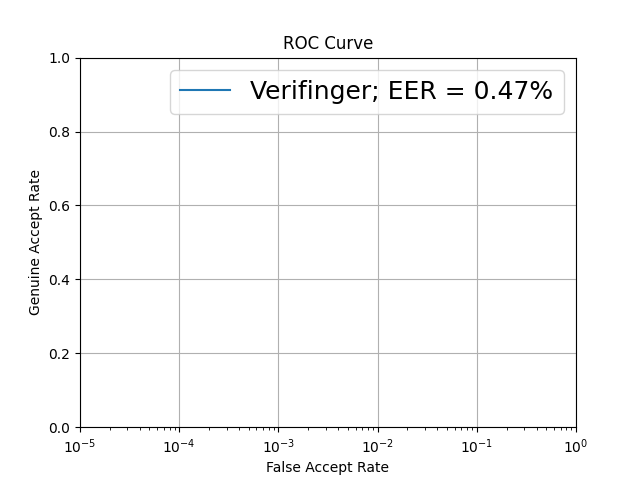
\includegraphics[width=1.74in]{Figure/26-08-2022/ending-193-bifurcation-62.png}%
    \label{ending-193-bifurcation-62}}
    \subfloat[]{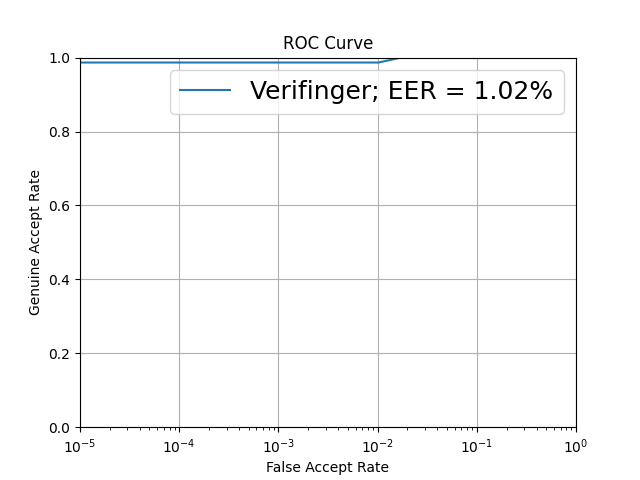
\includegraphics[width=1.74in]{Figure/26-08-2022/ending-96-bifurcation-31.png}%
    \label{ending-96-bifurcation-31}}
    \subfloat[]{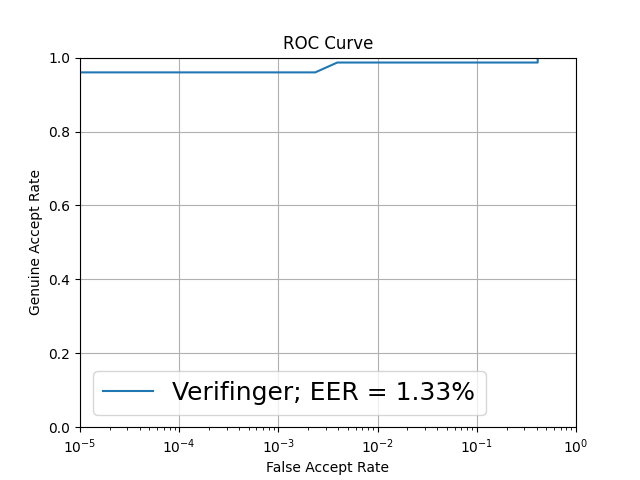
\includegraphics[width=1.74in]{Figure/26-08-2022/ending-48-bifurcation-15.png}%
    \label{ending-48-bifurcation-15}}
    \subfloat[]{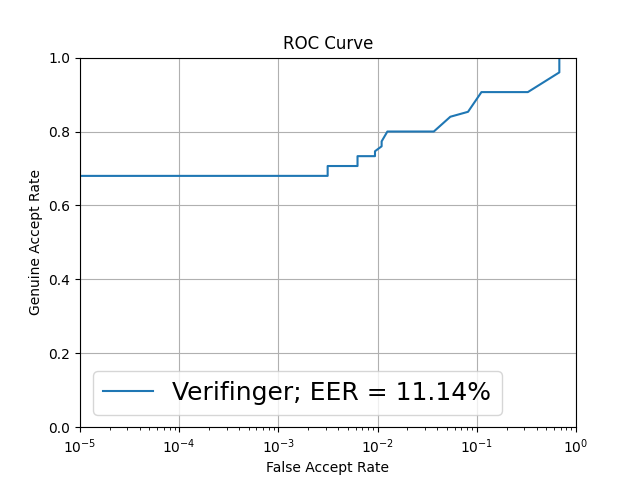
\includegraphics[width=1.74in]{Figure/26-08-2022/ending-24-bifurcation-7.png}%
    \label{ending-24-bifurcation-7}}
    
    \caption{The ROC is generated by recombining the minutiae texts by changing the number of endings and bifurcations. As for the number of ending points and bifurcations, it follows the Table \ref{original-text-table}.}
    \label{original-text}
    % \vspace{-0.4cm}
\end{figure}


We can clearly get a conclusion that the ending has a greater impact on matching accuracy than the bifurcation. For example, with the same 64, 32 and 16 minutiae, the matching accuracy of only ending is much higher than the matching accuracy of only bifurcation. It stands to reason that bifurcation is more robust for matching problems, but here the results are the opposite, probably because bifurcation is not well labelled during training or the model detects inaccurate position of bifurcations.




\subsubsection{Normalize Angle Range}
The angle of detection for this blood vessel key points is [0, 180) and most of the directions are vertical, so the angle range is extended linearly to (0, 360] here, with the other value remaining the same as original result. Follow the previous experiments, the number of components of the minutiae was changed by changing the number of ending points and bifurcations, as the Table \ref{angle-text-table}. The ROC curves are showed on the Fig. \ref{angle-text}. One obvious change here is that changing the angle range improves detection accuracy for only-bifurcation matching performance, which can be compared with Table \ref{angle-text-table} and Table \ref{original-text-table}. However, for matching with only-ending or with both ending and bifurcation, the corresponding matching performance is reduced.

\begin{figure}[h!]
    \centering
    \subfloat[]{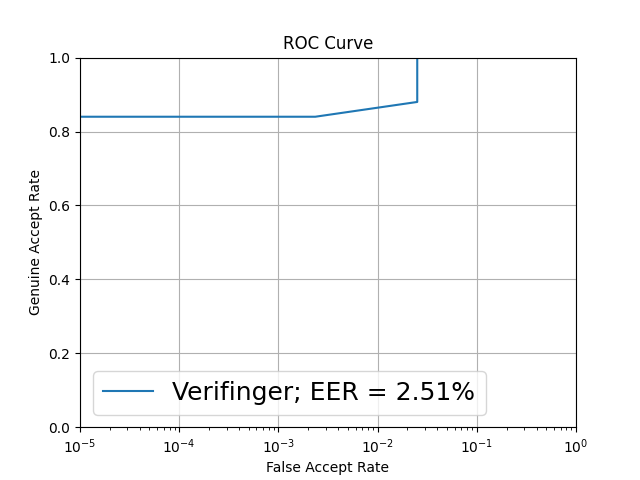
\includegraphics[width=1.74in]{Figure/26-08-2022/angle-ending-128-bifurcation-0.png}%
    \label{angle-ending-128-bifurcation-0}}
    \subfloat[]{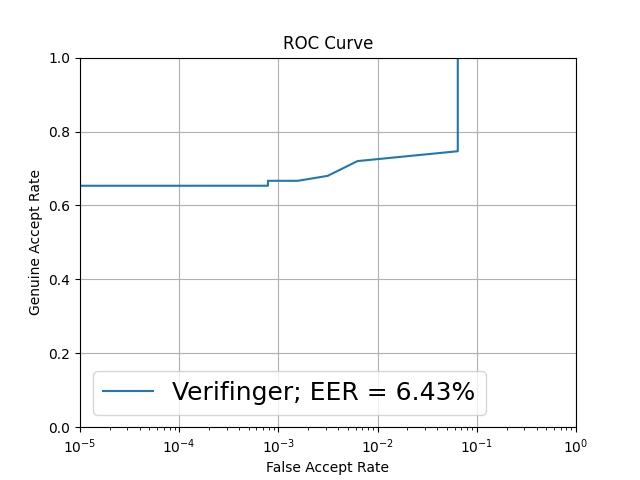
\includegraphics[width=1.74in]{Figure/26-08-2022/angle-ending-64-bifurcation-0.png}%
    \label{angle-ending-64-bifurcation-0}}
    \subfloat[]{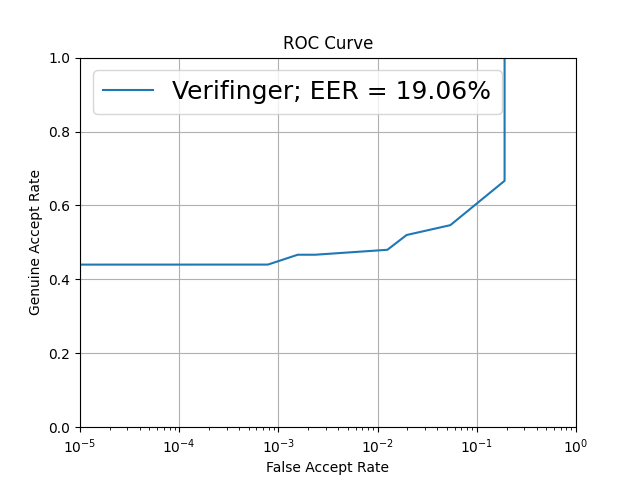
\includegraphics[width=1.74in]{Figure/26-08-2022/angle-ending-32-bifurcation-0.png}%
    \label{angle-ending-32-bifurcation-0}}
    \subfloat[]{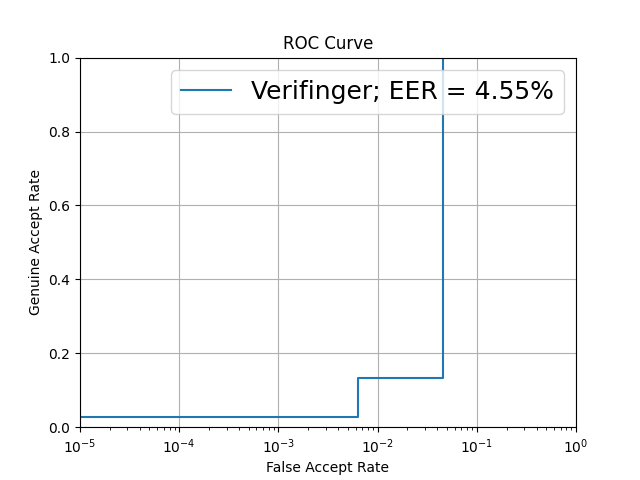
\includegraphics[width=1.74in]{Figure/26-08-2022/angle-ending-0-bifurcation-32.png}%
    \label{angle-ending-0-bifurcation-32}}

    \subfloat[]{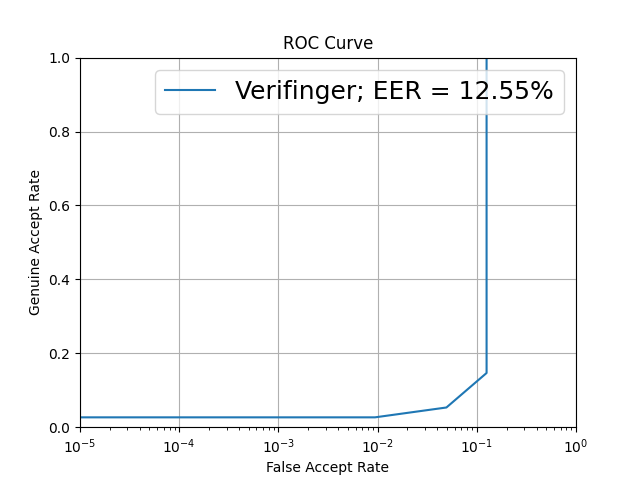
\includegraphics[width=1.74in]{Figure/26-08-2022/angle-ending-0-bifurcation-16.png}%
    \label{angle-ending-0-bifurcation-16}}
    \subfloat[]{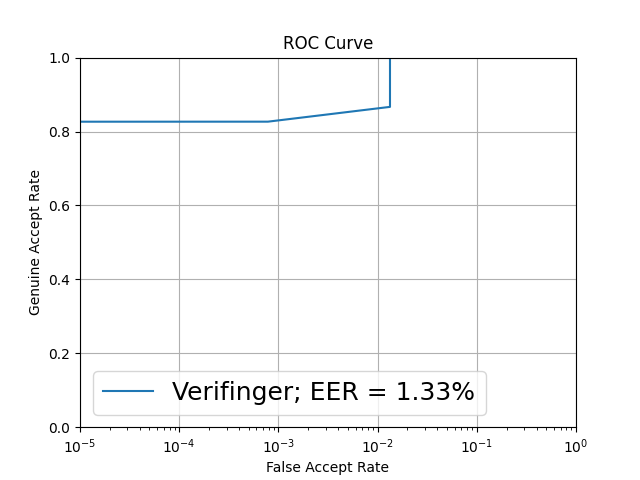
\includegraphics[width=1.74in]{Figure/26-08-2022/angle-ending-96-bifurcation-31.png}%
    \label{angle-ending-96-bifurcation-31}}
    \subfloat[]{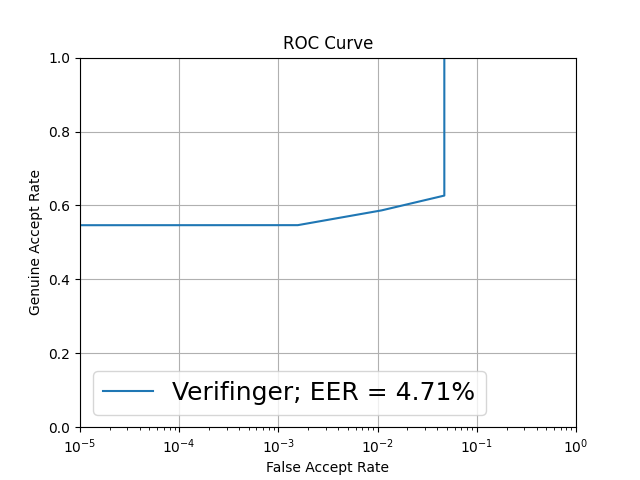
\includegraphics[width=1.74in]{Figure/26-08-2022/angle-ending-48-bifurcation-15.png}%
    \label{angle-ending-48-bifurcation-15}}
    
    \caption{The ROC is generated by recombining the minutiae texts by changing the number of endings and bifurcations, and by changing angle range to (0,360]. As for the number of ending points and bifurcations, it follows the Table \ref{angle-text-table}.}
    \label{angle-text}
    % \vspace{-0.4cm}
\end{figure}

\begin{table}[h!]
    \centering
    \caption{}
    \begin{tabular}{cccccc}
    \hline
    Angle Range & (x,y) Range  & Minutiae                    & EER     & DI   & Figure \\ \hline
    (0, 360{]}  & (1920, 1080) & Only 128 Ending             & 2.51\%  & 1.51 & Fig. \ref{angle-ending-128-bifurcation-0}  \\
    (0, 360{]}  & (1920, 1080) & Only 64 Ending              & 6.43\%  & 1.16 & Fig. \ref{angle-ending-64-bifurcation-0}  \\
    (0, 360{]}  & (1920, 1080) & Only 32 Ending              & 19.06\% & 0.96 & Fig. \ref{angle-ending-32-bifurcation-0}  \\
    (0, 360{]}  & (1920, 1080) & Only 62 Bifurcation         & 3.29\%  & 0.6  & Not draw  \\
    (0, 360{]}  & (1920, 1080) & Only 32 Bifurcation         & 4.55\%  & 0.3  & Fig. \ref{angle-ending-0-bifurcation-32}  \\
    (0, 360{]}  & (1920, 1080) & Only 16 Bifurcation         & 12.55\% & 0.21 & Fig. \ref{angle-ending-0-bifurcation-16}  \\
    (0, 360{]}  & (1920, 1080) & Ending: 96; Bifurcation: 32 & 1.33\%  & 1.33 & Fig. \ref{angle-ending-96-bifurcation-31} \\
    (0, 360{]}  & (1920, 1080) & Ending: 48; Bifurcation: 15 & 4.70\%  & 1.03 & Fig. \ref{angle-ending-48-bifurcation-15} \\
    (0, 360{]}  & (1920, 1080) & Ending: 24; Bifurcation: 7  & 13.57\% & 0.87 & Not draw \\ \hline
    \end{tabular}
    \label{angle-text-table}
\end{table}


\subsubsection{Normalize Angle Range and (X, Y) Range}
\begin{table}[ht!]
    \centering
    \caption{}
    \begin{tabular}{cccccc}
    \hline
    Angle Range & (x,y) Range & Minutiae                    & EER     & DI   & Figure \\ \hline
    (0, 360{]}  & (384, 216)  & Only 128 Ending             & 11.14\% & 1.51 & Fig. \ref{angle-xy-ending-128-bifurcation-0}  \\
    (0, 360{]}  & (384, 216)  & Only 64 Ending              & 10.82\% & 1.46 & Fig. \ref{angle-xy-ending-64-bifurcation-0}  \\
    (0, 360{]}  & (384, 216)  & Only 32 Ending              & 21.57\% & 1.31 & Fig. \ref{angle-xy-ending-32-bifurcation-0}  \\
    (0, 360{]}  & (384, 216)  & Only 62 Bifurcation         & 22.35\% & 1.1  & Fig. \ref{angle-xy-ending-0-bifurcation-62}  \\
    (0, 360{]}  & (384, 216)  & Only 32 Bifurcation         & 32.34\% & 0.81 & Fig. \ref{angle-xy-ending-0-bifurcation-32}  \\
    (0, 360{]}  & (384, 216)  & Ending: 96; Bifurcation: 32 & 11.61\% & 1.71 & Fig. \ref{angle-xy-ending-96-bifurcation-31} \\
    (0, 360{]}  & (384, 216)  & Ending: 48; Bifurcation: 15 & 16.16\% & 1.66 & Fig. \ref{angle-xy-ending-48-bifurcation-15} \\
    (0, 360{]}  & (384, 216)  & Ending: 24; Bifurcation: 7  & 27.92\% & 1.13 & Not draw \\ \hline
    \end{tabular}
    \label{angle-xy-text-table}
\end{table}

\begin{figure}[ht!]
    \centering
    \subfloat[]{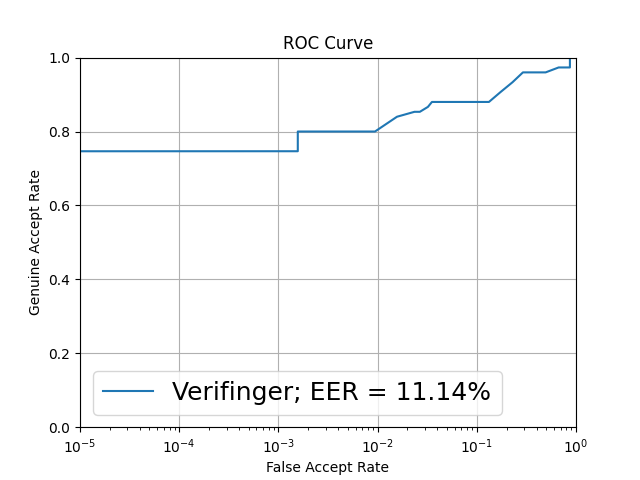
\includegraphics[width=1.74in]{Figure/26-08-2022/angle-xy-ending-128-bifurcation-0.png}%
    \label{angle-xy-ending-128-bifurcation-0}}
    \subfloat[]{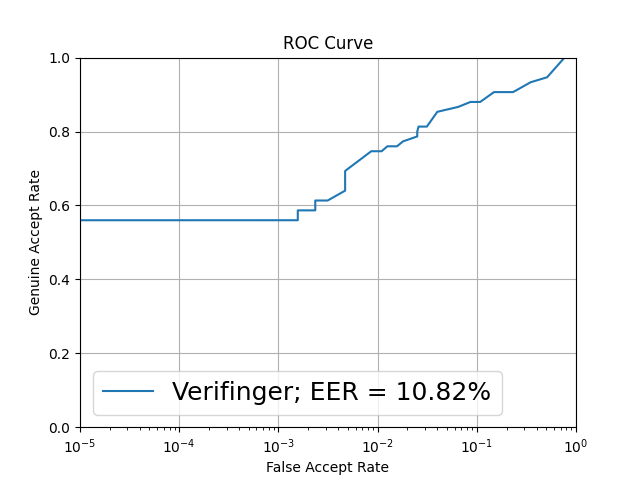
\includegraphics[width=1.74in]{Figure/26-08-2022/angle-xy-ending-64-bifurcation-0.png}%
    \label{angle-xy-ending-64-bifurcation-0}}
    \subfloat[]{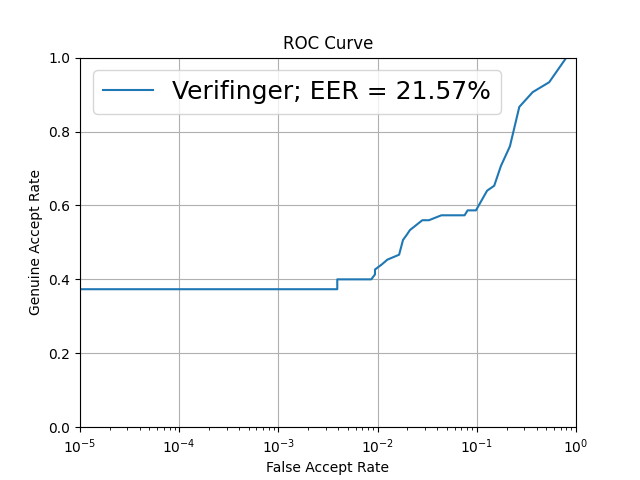
\includegraphics[width=1.74in]{Figure/26-08-2022/angle-xy-ending-32-bifurcation-0.png}%
    \label{angle-xy-ending-32-bifurcation-0}}
    \subfloat[]{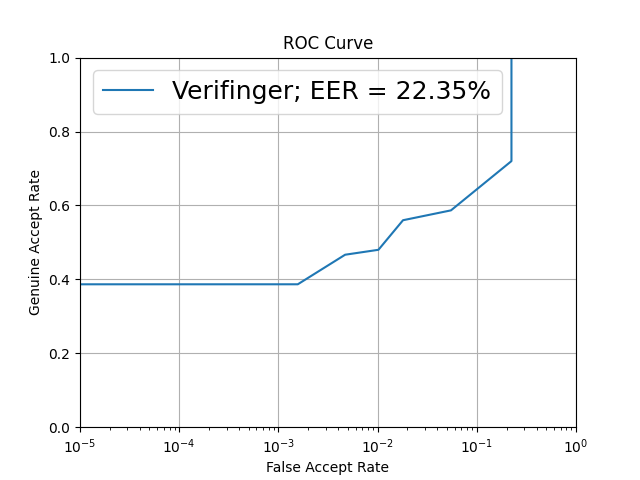
\includegraphics[width=1.74in]{Figure/26-08-2022/angle-xy-ending-0-bifurcation-62.png}%
    \label{angle-xy-ending-0-bifurcation-62}}

    \subfloat[]{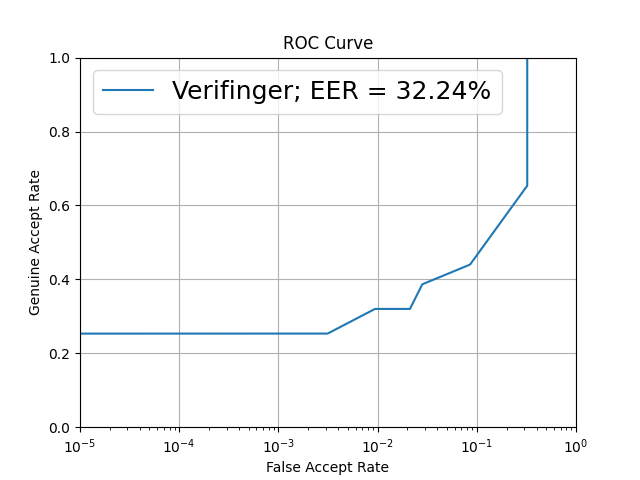
\includegraphics[width=1.74in]{Figure/26-08-2022/angle-xy-ending-0-bifurcation-32.png}%
    \label{angle-xy-ending-0-bifurcation-32}}
    \subfloat[]{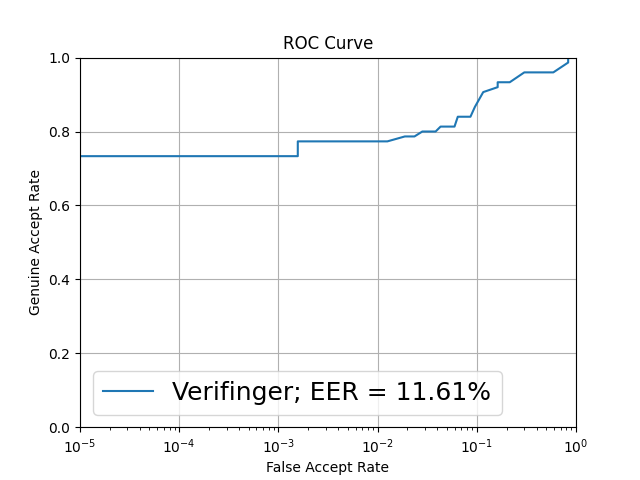
\includegraphics[width=1.74in]{Figure/26-08-2022/angle-xy-ending-96-bifurcation-31.png}%
    \label{angle-xy-ending-96-bifurcation-31}}
    \subfloat[]{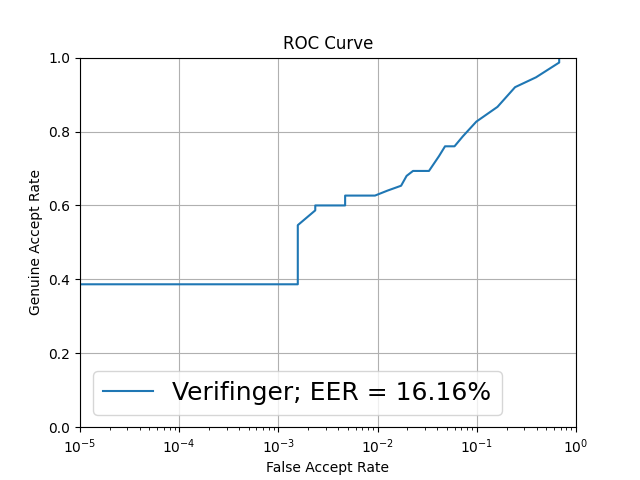
\includegraphics[width=1.74in]{Figure/26-08-2022/angle-xy-ending-48-bifurcation-15.png}%
    \label{angle-xy-ending-48-bifurcation-15}}
    
    \caption{The ROC is generated by recombining the minutiae texts by changing the number of endings and bifurcations, by changing angle range to (0,360], and by chaning the (x, y) range. As for the number of ending points and bifurcations, it follows the Table \ref{angle-xy-text-table}.}
    \label{angle-xy-text}
    % \vspace{-0.4cm}
\end{figure}

Finally, we scaled the range of detected coordinates equally. The size of the image we detected was 1920x1080, so the corresponding detected position was in the range. By looking the normal fingerprint minutiae coordinates values, they are all less than 400, so there the coordinate range is changed by 1920/5=384 and 1080/5=216. But as you can see by the Table \ref{angle-xy-text-table} and the Fig. \ref{angle-xy-text}, changing the coordinate range makes all the matching performance drop.



